% Source for the figure of ConcurrentCuckooTable (sec. 24.7): a table of 16
% buckets in 4 regions of 4 buckets, each region with the version of its
% lock (odd while held); the two buckets of a key lie in its region.
% Build: make figures (in ../build).
\documentclass[border=4pt]{standalone}
\usepackage[T1]{fontenc}
\usepackage{newpxtext,newpxmath}
\usepackage[varqu,varl,scaled=0.95]{zi4}
\usepackage{tikz}
% tikz-ads.tex: the TikZ styles shared by the figures of the memory of the
% manual, \input by each standalone figure: a cell of a vector (cell), the
% cell that an operation touches (touched), a free cell (free), a node of a
% linked structure (node), the labels of indices (index) and of variables
% (var), a pointer (ptr), and \cells and \indices to draw a row of cells.
\usetikzlibrary{arrows.meta,positioning,calc,fit,shapes.multipart}
\definecolor{adsTouched}{RGB}{214,196,236}
\definecolor{adsFree}{RGB}{236,236,236}
\tikzset{
  ads/.style={>={Stealth[length=2mm]},font=\small,
              every node/.append style={inner sep=0pt}},
  cell/.style={draw,minimum width=7mm,minimum height=7mm,
               font=\small\ttfamily,outer sep=0pt},
  touched/.style={cell,fill=adsTouched},
  free/.style={cell,fill=adsFree,text=black!45},
  node/.style={draw,rounded corners=1pt,minimum width=8mm,
               minimum height=6mm,font=\small\ttfamily},
  index/.style={font=\scriptsize\ttfamily,text=black!60},
  var/.style={font=\small\itshape},
  ptr/.style={->,thick}
}
% \cells{name}{x,y}{list}: a row of cells, the first at (x,y), named
% name-0, name-1, ...; each item is text/style, the style one of cell,
% touched and free (e.g., {a/cell,e/touched,/free})
\newcommand{\cells}[3]{%
  \foreach \v/\s [count=\i from 0] in {#3}
    \node[\s] (#1-\i) at ($(#2)+(\i*7mm,0)$) {\v};}
% \indices{name}{n}: the indices 0 .. n-1 under the cells of name
\newcommand{\indices}[2]{%
  \foreach \i in {0,...,\numexpr#2-1\relax}
    \node[index,below=1.2mm of #1-\i] {\i};}

\usetikzlibrary{decorations.pathreplacing}
\begin{document}
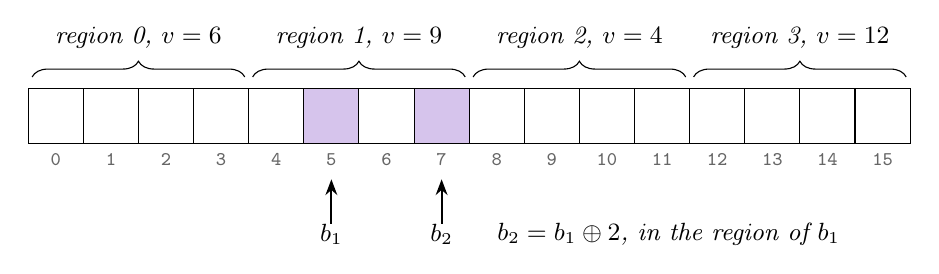
\begin{tikzpicture}[ads]
  \cells{B}{0,0}{/cell,/cell,/cell,/cell,/cell,/touched,/cell,/touched,/cell,/cell,/cell,/cell,/cell,/cell,/cell,/cell}
  \indices{B}{16}
  \foreach \a/\b/\r/\v in {0/3/0/6,4/7/1/9,8/11/2/4,12/15/3/12} {
    \draw[decorate,decoration={brace,amplitude=2mm}]
      ($(B-\a.north west)+(0.5mm,1.5mm)$) --
      ($(B-\b.north east)+(-0.5mm,1.5mm)$)
      node[midway,above=3.5mm,var] {region \r, $v = \v$};
  }
  \node[var] (b1) at ($(B-5)+(0,-15mm)$) {$b_1$};
  \node[var] (b2) at ($(B-7)+(0,-15mm)$) {$b_2$};
  \draw[ptr] (b1) -- ($(B-5.south)+(0,-4.5mm)$);
  \draw[ptr] (b2) -- ($(B-7.south)+(0,-4.5mm)$);
  \node[var,anchor=west] at ($(B-8)+(0,-15mm)$) {$b_2 = b_1 \oplus 2$, in the region of $b_1$};
\end{tikzpicture}
\end{document}
